\section{DIỆN TÍCH XUNG QUANH VÀ THỂ TÍCH CỦA HÌNH CHÓP TAM GIÁC ĐỀU, HÌNH CHÓP TỨ GIÁC ĐỀU}

\subsubsection{Kiến thức trọng tâm}
\subsection{Diện tích xung quanh của hình chóp tam giác đều và hình chóp tứ giác đều}
\begin{boxdn}
	Diện tích xung quanh của hình chóp tam giác đều (hình chóp tứ giác đều) bằng tổng diện tích của các mặt bên.
\end{boxdn}
\begin{note}
	Diện tích toàn phần của hình chóp tam giác đều (hình chóp tứ giác đều) bằng tổng của diện tích xung quanh và diện tích đáy:
	\[\rm S_{tp}= S_{xq}+ S_{\text{đáy}}\]
	($\rm S_{tp}$ là diện tích toàn phần, $\rm S_{xq}$ là diện tích xung quanh, $\rm S_{\text{đáy}}$ là diện tích đáy)
\end{note}

\subsection{Thể tích của hình chóp tam giác đều và hình chóp tứ giác đều}
\begin{boxdn}
	Thể tích của hình chóp tam giác đều (hình chóp tứ giác đều) bằng $\dfrac{1}{3}$ diện tích đáy nhân với chiều cao.
	\[\rm V=\dfrac{1}{3}\cdot S_{\text{đáy}}\cdot h\]
	($\rm V$ là thể tích, $\rm S_{\text{đáy}}$ là diện tích đáy và $\rm h$ là chiều cao).
\end{boxdn}

\begin{vd}%[Dự án EX-8-Đề Cương Toán 8]%[Phạm Minh Khánh]%[8H1N2-1]
	\immini{
		Một tấm bìa gấp thành hình chóp tam giác đều với các mặt bên đều là hình tam giác đều. Với số đo trên hình vẽ, hãy tính diện tích xung quanh và diện tích toàn phần của hình này.
	}
	{
		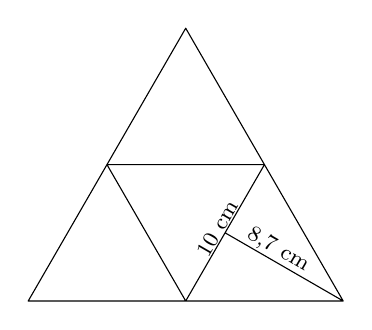
\begin{tikzpicture}[line cap=round, line join=round, font=\footnotesize, scale=1]
			\def\a{4}
			\path (0,0) coordinate (O)
			(0:\a) coordinate (A)
			(60:\a) coordinate (B) 
			(barycentric cs:O=1,A=1) coordinate (M)
			(barycentric cs:A=1,B=1) coordinate (N)
			(barycentric cs:B=1,O=1) coordinate (P)
			;
			\draw (O)--(A)--(B)--cycle
			(M)--(N) node[above=-1mm,pos=.5,sloped]{10 cm}--(P)--cycle
			(barycentric cs:M=1,N=1)--(A) node[above=-1mm,pos=.4,sloped]{8{,}7 cm}
			;
	\end{tikzpicture}}
	\loigiai{
		\begin{itemize}
			\item Diện tích xung quanh: $\rm S_{xq}=3\cdot\dfrac{1}{2}\cdot10\cdot8{,}7=130{,}5$ ($\rm cm^2$)
			\item Diện tích toàn phần: $\rm S_{tp}=4\cdot\dfrac{1}{2}\cdot10\cdot8{,}7=174$ ($\rm cm^2$)
		\end{itemize}
	}
\end{vd}

\begin{vd}%[Dự án EX-8-Đề Cương Toán 8]%[Phạm Minh Khánh]%[8H1N2-1]
	Nam làm một chiếc hộp hình chóp tứ giác đều như Hình a, sau đó Nam trải các mặt của chiếc hộp với các số đo đã cho như Hình b.
	\begin{center}
		\begin{tikzpicture}[scale=1, font=\footnotesize, line join=round, line cap=round, >=stealth]
			\def\bc{3}
			\def\ba{2}
			\def\h{4}
			\def\gocB{30}
			\coordinate (B) at (0,0);
			\coordinate (A) at (\gocB:\ba);
			\coordinate (C) at (\bc,0);
			\coordinate (D) at ($(C)-(B)+(A)$);
			\coordinate (O) at ($(A)!.5!(C)$);
			\coordinate (S) at ($(O)+(90:\h)$);
			\draw[black,fill=yellow!50!black] (S)--(B)--(C);
			\draw[black,fill=yellow!90!black] (S)--(C)--(D);
			\path (0.5*\bc+0.8,0) node[below=4mm]{a)};
		\end{tikzpicture}
		\hspace*{1cm}	
		\begin{tikzpicture}[line cap=round, line join=round, font=\footnotesize, scale=1]
			\path
			(5.5,1) coordinate (a)
			(5.5,-1) coordinate (b)
			(7.5,-1) coordinate (c)
			($(a)+(c)-(b)$) coordinate (d)
			(3,0) coordinate (ha)
			(6.5,-3.5) coordinate (hb)
			(10,0) coordinate (hc)
			(6.5,3.5) coordinate (hd)
			(barycentric cs:a=1,b=1) coordinate (mab)
			(barycentric cs:b=1,c=1) coordinate (mbc)
			(barycentric cs:c=1,d=1) coordinate (mcd)
			(barycentric cs:d=1,a=1) coordinate (mda)
			;
			\draw[fill=white] (a)--(ha)--(b)--(hb)--(c)--(hc)--(d)--(hd)--cycle;
			\draw (b)--(a) node[below=-1mm,pos=.5,sloped]{4 cm}
			(b)--(c) node[above=-1mm,pos=.5,sloped]{4 cm}
			(c)--(d) node[above=-1mm,pos=.5,sloped]{4 cm}
			(d)--(a) node[below=-1mm,pos=.5,sloped]{4 cm}
			(ha)--(mab) node[above=-1mm,pos=.6,sloped]{5 cm}
			(mcd)--(hc) node[above=-1mm,pos=.4,sloped]{5 cm}
			(hb)--(mbc) node[above=-1mm,pos=.6,sloped]{5 cm}
			(mda)--(hd) node[above=-1mm,pos=.4,sloped]{5 cm}
			;
			\draw 	pic[draw,angle radius=2.5mm]{right angle=ha--mab--b}
			pic[draw,angle radius=2.5mm]{right angle=hb--mbc--c}
			pic[draw,angle radius=2.5mm]{right angle=hc--mcd--d}
			pic[draw,angle radius=2.5mm]{right angle=hd--mda--a};
			\path (6.5,-3.75) node[below]{b)};
		\end{tikzpicture}
	\end{center}
	Tính diện tích xung quanh và diện tích toàn phần của chiếc hộp hình chóp tứ giác đều ở Hình a trên.
	\loigiai{
		Diện tích xung quanh của chiếc hộp: $\rm S_{xq}=4\cdot\dfrac{1}{2} \cdot 4 \cdot 5=40 $ ($\rm cm^2$). \\
		Diện tích toàn phần của chiếc hộp: $\rm S_{tp}=S_{xq}+S_{\text{đáy}} =40+4\cdot4=56$ $(\rm cm^2)$.
	}
\end{vd}

\begin{vd}%[Dự án EX-8-Đề Cương Toán 8]%[Phạm Minh Khánh]%[8H1H2-1]
	Cho một hình chóp tứ giác đều có chiều cao của tam giác mặt bên kẻ từ đỉnh của hình chóp bằng $5 \mathrm{~cm}$ và diện tích xung quanh bằng $30 \mathrm{~cm}^2$. Tính độ dài cạnh đáy của hình chóp đó.
	\loigiai{
		Gọi độ dài cạnh đáy của hình chóp tứ giác đều đó là $x \mathrm{~cm}$. Ta có:
		$$S_{x q}=\dfrac{1}{2} \cdot(x.4) \cdot 5.$$
		Do đó $x=\dfrac{2S_{xq}}{4\cdot 5}=\dfrac{2\cdot 30}{4\cdot 5}=3\mathrm{~(cm)}$.\\
		Vậy hình chóp có độ dài cạnh đáy là $3\mathrm{~(cm)}$.
	}
\end{vd}

\begin{vd}%[Dự án EX-8-Đề Cương Toán 8]%[Phạm Minh Khánh]%[8H1N2-2]
	\immini{
		Tính thể tích của hình chóp tam giác đều, biết chiều cao của hình chóp là $\rm 4\,cm$, tam giác đáy có cạnh $\rm 6\,cm$ và chiều cao $\rm 3\sqrt{3}\,cm$.}{
		\begin{tikzpicture}[line cap=round, line join=round, font=\footnotesize, scale=0.8]
			\def\a{6} \def\h{4}
			\path 	(0:0) coordinate (A)
			++(0:\a) coordinate (B)
			++(-135:\a/2) coordinate (C)
			($(C)!0.5!(B)$) coordinate (M)
			($(A)!2/3!(M)$) coordinate (H)
			($(H)+(90:\h)$) coordinate (S);
			\draw (C)--(A) (C)--(B)
			(A)--(S)	(B)--(S)	(C)--(S);
			\draw[dashed] (M)--(A)--(B) (S)--(H) ;
			\draw pic[draw,angle radius=3mm]{right angle=S--H--A}
			pic[draw,angle radius=3mm]{right angle=A--M--B};
			\path 	(A)--(C) node[below,pos=.5,sloped]{6 cm}
			(A)--(M) node[below,pos=.65,sloped]{$3\sqrt{3}$ cm}
			(S)--(H) node[above,pos=.6,sloped]{4 cm} 
			;	
		\end{tikzpicture}
	}
	\loigiai{
		Diện tích đáy của hình chóp tam giác đều:
		\[\rm S_{\text{đáy}}=\dfrac{1}{2}\cdot6\cdot3\sqrt{3} =9\sqrt{3}\,(cm^2)\]
		Thể tích của hình chóp tam giác đều là
		\[\rm V=\dfrac{1}{3}\cdot S_{\text{đáy}}\cdot h =\dfrac{1}{3}\cdot9\sqrt{3}\cdot4=12\sqrt{3}\,(cm^3).\] 
	}
\end{vd}

\begin{vd}%[Dự án EX-8-Đề Cương Toán 8]%[Phạm Minh Khánh]%[8H1H2-2]
	Một khối chóp tam giác đều có thể tích là $50$ cm$^3$, diện tích đáy $30\mathrm{~cm^2}$. Tính chiều cao của khối chóp đó.
	\loigiai{
		Ta có $V = \dfrac{1}{3} Sh$. Do đó $h=\dfrac{3V}{S}=\dfrac{3\cdot 50}{30}=5\mathrm{~(cm)}$.\\
		Vậy chiều cao của khối chóp đó là $5\mathrm{~(cm)}$. 
	}
\end{vd}

\begin{vd}%[Dự án EX-8-Đề Cương Toán 8]%[Phạm Minh Khánh]%[8H1H2-2]
	\immini{
		Tính thể tích của hình chóp tứ giác đều có chiều cao $\rm 3\,cm$, độ dài cạnh của tứ giác đáy là $\rm 5\, cm$.
	}{	
		\begin{tikzpicture}[line cap=round, line join=round, font=\footnotesize, scale=1]
			\def\a{3} \def\h{2.5}
			\path 	(0:0) coordinate (A)
			++(0:\a) coordinate (D)
			++(-110:\a/2) coordinate (C)
			($(A)+(C)-(D)$) coordinate (B)
			(intersection of A--C and B--D) coordinate (O)
			($(O)+(90:\h)$) coordinate (S);
			\draw[dashed] 	(C)--(A)--(D)--(B) (S)--(O)	;
			\draw (B)--(C)--(D)--(S)--(A)--(B)--(S)--(C);	
			\draw pic[draw,angle radius=3mm]{right angle=B--O--S};	
			\path (B)--(C) node[above,pos=.5]{5 cm} 
			(S)--(O) node[above,pos=.78,sloped]{3 cm}
			;
	\end{tikzpicture} } 
	\loigiai{
		Thể tích của hình chóp tứ giác đều (hình 4) là\\
		\centerline{
			$\rm V=\dfrac{1}{3}\cdot S_{\text{đáy}}\cdot h =\dfrac{1}{3}\cdot5^2\cdot3=25\,(cm^3).$} 
	}
\end{vd}

\begin{vd}%[Dự án EX-8-Đề Cương Toán 8]%[Phạm Minh Khánh]%[8H1H2-2]
	Một khối chóp tam giác đều có thể tích là $100$ cm$^3$, chiều cao là $15\mathrm{~cm}$. Tính diện tích đáy của khối chóp đó.
	\loigiai{
		Ta có $V = \dfrac{1}{3} Sh$. Do đó $S=\dfrac{3V}{h}=\dfrac{3\cdot 100}{15}=20\mathrm{~(cm)}$.\\ Vậy chiều cao của khối chóp đó là $20\mathrm{~(cm)}$. 
	}
\end{vd}

\begin{vd}%[Dự án EX-8-Đề Cương Toán 8]%[Phạm Minh Khánh]%[8H1H2-2]
	Một khối chóp tứ giác đều có thể tích là $70$ cm$^3$, diện tích đáy $20\mathrm{~cm^2}$. Tính chiều cao của khối chóp đó.
	\loigiai{
		Ta có $V = \dfrac{1}{3} Sh$. Do đó $h=\dfrac{3V}{S}=\dfrac{3\cdot 70}{20}=10{,}5\mathrm{~(cm)}$.\\
		Vậy chiều cao của khối chóp đó là $10{,}5\mathrm{~(cm)}$. 
	}
\end{vd}

\begin{vd}%[Dự án EX-8-Đề Cương Toán 8]%[Phạm Minh Khánh]%[8H1H2-3]
	\immini{
		Một cái lều bằng vải có dạng hình chóp tam giác đều với độ dài cạnh đáy $3 \mathrm{~m}$ và chiều cao của tam giác mặt bên kẻ từ đỉnh của hình chóp bằng $2{,}2 \mathrm{~m}$. Biết rằng mép may là không đáng kể và cứ mỗi mét vuông vải có giá $ 50 000$ đồng. Tính số tiền vải cần dùng để phủ quanh chiếc lều đó. 
	}{
		\begin{tikzpicture}[scale=1, font=\footnotesize, line join=round, line cap=round, >=stealth,scale=0.8]
			\def\ac{6}
			\def\ab{3}
			\def\h{4}
			\def\gocA{30}
			\coordinate (A) at (0,0);
			\coordinate (C) at (\ac,0);
			\coordinate (B) at (-\gocA:\ab);
			\coordinate (M) at ($(B)!.5!(A)$);
			\coordinate (G) at ($(C)!2/3!(M)$);
			\coordinate (S) at ($(G)+(90:\h)$);
			\draw[fill=green!20] (A)--(B)--(C)--(S)--cycle; 
			\draw (M)--(S)--(B);
			\draw pic[draw=black,angle radius=5pt] {right angle = S--M--B}; 
			\path (S)--(M)node[blue,midway,above,sloped]{$2{,}2\mathrm{~m}$}
			(B)--(C)node[blue,midway,below,sloped]{$3\mathrm{~m}$}
			;
			\draw[dashed] (A)--(C);
		\end{tikzpicture}
	}
	\loigiai{
		Diện tích xung quanh của lều là
		$$S_{xq}=\dfrac{1}{2}\cdot (3\cdot 3)\cdot 2{,}2=9{,}9\mathrm{~(cm^2)}.$$
		Số tiền cần phải trả để hoàn thành việc sơn phủ là
		$$50 000\cdot 9{,}9=495 000 \text{ đồng.}$$
	}
\end{vd}

\begin{vd}%[Dự án EX-8-Đề Cương Toán 8]%[Phạm Minh Khánh]%[8H1H2-3]
	\immini{
		Một mái che giếng trời có dạng hình chóp tứ giác đều với độ dài cạnh đáy khoảng $2{,}2 \mathrm{~m}$ và chiều cao của tam giác mặt bên kẻ từ đỉnh của hình chóp khoảng $2{,}8 \mathrm{~m}$ (Hình bên). Cần phải trả bao nhiêu tiền để làm mái che giếng trời đó? Biết rằng giá để làm mỗi mét vuông mái che được tính là $1 800 000$ đồng (bao gồm tiền vật liệu và tiền công).
	}{
		\begin{tikzpicture}[scale=0.7, font=\footnotesize, line join=round, line cap=round, >=stealth]
			\def\bc{4}
			\def\ba{3}
			\def\h{4}
			\def\gocB{30}
			\coordinate (B) at (0,0);
			\coordinate (A) at (\gocB:\ba);
			\coordinate (C) at (\bc,0);
			\coordinate (D) at ($(C)-(B)+(A)$);
			\coordinate (O) at ($(A)!.5!(C)$);
			\coordinate (H) at ($(D)!.5!(C)$);
			\coordinate (S) at ($(O)+(90:\h)$);
			\draw[fill=green!20] (B)--(C)--(D)--(S)--cycle; 
			\draw (S)--(C);
			\draw[dashed] (A)--(D) (S)--(A)--(B);
			\foreach \diem in {A,B,C,D,S}	\fill (\diem)circle(1.5pt);
		\end{tikzpicture}
	}
	\loigiai{
		Diện tích xung quanh của cái giếng trời là
		$S_{xq}=\dfrac{1}{2}\cdot (2{,}2\cdot 4)\cdot 2{,}8=12{,}32\mathrm{~(m^2)}.$\\
		Số tiền cần phải trả để hoàn thành việc sơn phủ là
		$1 800 000\cdot 12{,}32=22 176 000 \text{ đồng.}$
	}
\end{vd}

\begin{vd}%[Dự án EX-8-Đề Cương Toán 8]%[Phạm Minh Khánh]%[8H1H2-3]
	\immini{
		Một kho chứa có dạng hình chóp tứ giác đều với độ dài cạnh đáy $6 \mathrm{~m}$ và chiều cao của tam giác mặt bên kẻ từ đỉnh của hình chóp bằng $3 \mathrm{~m}$. Người ta muốn sơn phủ bên ngoài cả ba mặt xung quanh của kho chứa đó và không sơn phủ phần làm cửa có diện tích là $3 \mathrm{~m}^2$. Biết rằng cứ mỗi mét vuông sơn cần trả $40 000$ đồng. Cần phải trả bao nhiêu tiền để hoàn thành việc sơn phủ đó?
	}{
		\begin{tikzpicture}[scale=1, font=\footnotesize, line join=round, line cap=round, >=stealth]
			\def\ac{4}
			\def\ab{1.5}
			\def\h{3}
			\def\gocA{35}
			\coordinate (A) at (0,0);
			\coordinate (D) at (\ac,0);
			\coordinate (B) at (-\gocA:\ab);
			\coordinate (C) at ($(B)+(D)-(A)$);
			\coordinate (M) at ($(B)!.5!(A)$);
			\coordinate (G) at ($(C)!1/2!(A)$);
			\coordinate (S) at ($(G)+(90:\h)$);
			\draw[fill=magenta!20] (A)--(B)--(C)--(S)--cycle; 
			\draw (M)--(S)--(B);
			\draw pic[draw=black,angle radius=5pt] {right angle = S--M--B}; 
			\path (S)--(M)node[blue,midway,above,sloped]{$3\mathrm{~m}$}
			(B)--(A)node[blue,midway,below,sloped]{$6\mathrm{~m}$}
			;
			\draw[dashed] (A)--(D)--(C) (S)--(D);
			\coordinate (N) at ($(B)!.5!(C)$);
			\coordinate (N') at ($(N)!.22!(S)$);
			\coordinate (pp) at ($($(N)!0.12!(B)$)!2!(N')$);
			\coordinate (tt) at ($($(N)!0.12!(C)$)!2!(N')$);
			\draw[fill=white] ($(N)!0.12!(B)$)--($(N)!0.12!(C)$)--(pp)--(tt)--cycle;
		\end{tikzpicture}
	}
	\loigiai{
		Diện tích cần sơn của kho là
		$$S_{xq}=\dfrac{1}{2}\cdot (6\cdot 4)\cdot 3-3=33\mathrm{~(cm^2)}.$$
		Số tiền cần phải trả để hoàn thành việc sơn phủ là
		$$40 000\cdot 33=1 320 000 \text{ đồng.}$$
	}
\end{vd}

\subsubsection{Bài tập}

\begin{bt}%[Dự án EX-8-Đề Cương Toán 8]%[Phạm Minh Khánh]%[8H1N2-1]
	\immini{
		Tính diện tích xung quanh của hình chóp tam giác đều $S.ABC$ trong hình vẽ bên.
	}{
		\begin{tikzpicture}[scale=1, font=\footnotesize, line join=round, line cap=round, >=stealth]
			\def\ac{4}
			\def\ab{2}
			\def\h{3}
			\def\gocA{50}
			\coordinate[label=left:$A$] (A) at (0,0);
			\coordinate[label=right:$C$] (C) at (\ac,0);
			\coordinate[label=below left:$B$] (B) at (-\gocA:\ab);
			\coordinate[label=below right:$H$] (M) at ($(B)!.5!(C)$);
			\coordinate (G) at ($(A)!2/3!(M)$);
			\coordinate[label=above:$S$] (S) at ($(G)+(90:\h)$);
			\draw (A)--(B)--(C)--(S)--cycle (M)--(S)--(B);
			\draw[dashed] (A)--(C);
			\foreach \diem in {A,B,C,S,M}	\fill (\diem)circle(1.5pt);
			\draw pic[draw=black,angle radius=5pt] {right angle = S--M--C};
			\path (A)--(B)node[blue,midway,above,sloped]{$5\mathrm{~cm}$}
			(S)--(M)node[blue,midway,above,sloped]{$6\mathrm{~cm}$}
			;
		\end{tikzpicture}
	}
	\loigiai{
		Diện tích xung quanh của hình chóp tam giác đều $S.ABC$ là
		$$
		S_{x q}=3\cdot\dfrac{1}{2}\cdot5\cdot 6=45\mathrm{~(cm^2)}.
		$$
	}
\end{bt}

\begin{bt}%[Dự án EX-8-Đề Cương Toán 8]%[Phạm Minh Khánh]%[8H1H2-1]
	\immini{
		Tính diện tích xung quanh của hình chóp tam giác đều $S.MNP$ trong hình vẽ bên, biết $I P=4 \mathrm{~cm}$ và trung đoạn $SI=6 \mathrm{~cm}$.
	}{
		\begin{tikzpicture}[scale=1, font=\footnotesize, line join=round, line cap=round, >=stealth]
			\def\ac{4}
			\def\ab{2}
			\def\h{3}
			\def\gocA{50}
			\coordinate[label=left:$N$] (A) at (0,0);
			\coordinate[label=right:$P$] (C) at (\ac,0);
			\coordinate[label=below left:$M$] (B) at (-\gocA:\ab);
			\coordinate[label=below right:$I$] (M) at ($(B)!.5!(C)$);
			\coordinate (G) at ($(A)!2/3!(M)$);
			\coordinate[label=above:$S$] (S) at ($(G)+(90:\h)$);
			\draw (A)--(B)--(C)--(S)--cycle (M)--(S)--(B);
			\draw[dashed] (A)--(C);
			\foreach \diem in {A,B,C,S,M}	\fill (\diem)circle(1.5pt);
			\draw pic[draw=black,angle radius=5pt] {right angle = S--M--C};
			\path (M)--(C)node[blue,midway,below,sloped]{$4\mathrm{~cm}$}
			(S)--(M)node[blue,midway,above,sloped]{$6\mathrm{~cm}$}
			;
		\end{tikzpicture}
	}
	\loigiai{
		Ta có $IP=4$ (cm), suy ra $MP=2IP=8$ cm.\\
		Diện tích xung quanh của hình chóp tam giác đều $S.MNP$ là
		$$
		S_{x q}=3\cdot \dfrac{1}{2}\cdot 8\cdot 6=72\mathrm{~(cm^2)}.
		$$
	}
\end{bt}

\begin{bt}%[Dự án EX-8-Đề Cương Toán 8]%[Phạm Minh Khánh]%[8H1N2-1]
	\immini{
		Tính diện tích xung quanh của hình chóp tứ giác đều $S.ABCD$ trong hình vẽ bên.
	}{
		\begin{tikzpicture}[scale=0.8, font=\footnotesize, line join=round, line cap=round, >=stealth]
			\def\bc{4}
			\def\ba{2}
			\def\h{4} 
			\def\gocB{30}
			\coordinate[label=below left:$B$] (B) at (0,0);
			\coordinate[label=above right:$A$] (A) at (\gocB:\ba);
			\coordinate[label=below:$C$] (C) at (\bc,0);
			\coordinate[label=right:$D$] (D) at ($(C)-(B)+(A)$);
			\coordinate (O) at ($(A)!.5!(C)$);
			\coordinate[label=below right:$H$] (H) at ($(D)!.5!(C)$);
			\coordinate[label=above:$S$] (S) at ($(O)+(90:\h)$);
			\draw (B)--(C)--(D)--(S)--cycle (H)--(S)--(C);
			\draw[dashed] (A)--(D) (S)--(A)--(B);
			\foreach \diem in {A,B,C,D,S}	\fill (\diem)circle(1.5pt);
			\draw pic[draw=black,angle radius=5pt] {right angle = S--H--D};
			\path (S)--(H) node[above,midway,sloped,blue]{$13\mathrm{~cm}$};
			\path (B)--(C) node[below,midway,sloped,blue]{$6\mathrm{~cm}$};
		\end{tikzpicture}
	}
	\loigiai{
		Diện tích xung quanh của hình chóp tứ giác đều $S.ABCD$ là
		$$
		S_{x q}=4\cdot\dfrac{1}{2}\cdot 6 \cdot 13=156\mathrm{~(cm^2)}.
		$$
	}
\end{bt}

\begin{bt}%[Dự án EX-8-Đề Cương Toán 8]%[Phạm Minh Khánh]%[8H1H2-1]
	\immini{
		Tính diện tích xung quanh của hình chóp tứ giác đều $S.MNPQ$ trong hình vẽ bên, biết $I Q=2 \mathrm{~cm}$ và trung đoạn $SI=5 \mathrm{~cm}$.
	}{
		\begin{tikzpicture}[scale=0.7, font=\footnotesize, line join=round, line cap=round, >=stealth]
			\def\bc{4}
			\def\ba{3}
			\def\h{4}
			\def\gocB{30}
			\coordinate[label=below left:$N$] (B) at (0,0);
			\coordinate[label=above right:$M$] (A) at (\gocB:\ba);
			\coordinate[label=below:$P$] (C) at (\bc,0);
			\coordinate[label=right:$Q$] (D) at ($(C)-(B)+(A)$);
			\coordinate (O) at ($(A)!.5!(C)$);
			\coordinate[label=below right:$I$] (H) at ($(D)!.5!(C)$);
			\coordinate[label=above:$S$] (S) at ($(O)+(90:\h)$);
			\draw (B)--(C)--(D)--(S)--cycle (H)--(S)--(C);
			\draw[dashed] (A)--(D) (S)--(A)--(B);
			\foreach \diem in {A,B,C,D,S}	\fill (\diem)circle(1.5pt);
			\draw pic[draw=black,angle radius=5pt] {right angle = S--H--D};
			\path (S)--(H) node[above,midway,sloped,blue]{$5\mathrm{~cm}$};
			\path (H)--(D) node[below,midway,sloped,blue]{$2\mathrm{~cm}$};
		\end{tikzpicture}
	}
	\loigiai{
		Ta có $IQ=2$ cm, suy ra $PQ=2IQ=4$ cm.\\
		Diện tích xung quanh của hình chóp tứ giác đều $S.MNPQ$ là
		$$
		S_{x q}=4\cdot\dfrac{1}{2}\cdot 4\cdot 5=40\mathrm{~(cm^2)}.
		$$
	}
\end{bt}

\begin{bt}%[Dự án EX-8-Đề Cương Toán 8]%[Phạm Minh Khánh]%[8H1H2-1]
	\immini	{Cho hình chóp tứ giác đều $S.ABCD$ như bên. 
		\begin{enumerate}
			\item Tính diện tích xung quanh của hình chóp.
			\item Tính diện tích toàn phần của hình chóp.
	\end{enumerate}}{
		\begin{tikzpicture}[line cap=round, line join=round, font=\footnotesize, scale=0.8, thick]
			\def\dai{4} \def\rong{2.75} \def\cao{3}
			\path 	(0:0) coordinate (A)
			++(0:\dai) coordinate (D)
			++(215:\rong) coordinate (C)
			($(A)+(C)-(D)$) coordinate (B)
			(intersection of A--C and B--D) coordinate (O)
			($(O)+(90:\cao)$) coordinate (S)
			(barycentric cs:C=1,D=1) coordinate (mCD);
			\draw[dashed] (B)--(A)--(D)--(B)	(O)--(S)--(A)--(C);
			\draw (B)--(C)--(D)--(S)--cycle (mCD)--(S)--(C);
			\foreach \x/\g in {A/135,B/-135,C/-45,D/45,S/90,O/-90}
			\fill[black] (\x) circle (1.5pt) ($(\g:3mm)+(\x)$) node {$\x$};	
			\draw pic[draw,angle radius=3mm]{right angle=D--mCD--S};	
			\path (B)--(C) node[below,pos=.5]{10 cm} 
			(S)--(mCD) node[above,pos=.6,sloped]{13 cm}
			;
	\end{tikzpicture}}
	\loigiai{	
		\begin{enumerate}
			\item Nửa chu vi đáy là $10\cdot 4 :2=20\left(\mathrm {cm}\right)$. 
			\\Diện tích xung quanh của hình chóp bằng $S_{\text{xq}}=p\cdot d=20\cdot 13=260\left(\mathrm {cm}^2\right)$. 
			\item Diện tích đáy của hình chóp là $10^2=100\left(\mathrm {cm}^2\right)$. 
			\\Diện tích toàn phần của hình chóp là $S_{tp}=260+100=360 \left(\mathrm {cm}^2\right)$.
	\end{enumerate}}
\end{bt}

\begin{bt}%[Dự án EX-8-Đề Cương Toán 8]%[Phạm Minh Khánh]%[8H1H2-1]
	Cho một hình chóp tam giác đều có độ dài cạnh đáy bằng $5 \mathrm{~cm}$, 
	chiều cao của tam giác mặt bên kẻ từ đỉnh của hình chóp bằng 
	$8 \mathrm{~cm}$. Tính diện tích xung quanh của hình chóp tam giác đều đó.
	\loigiai{
		Diện tích xung quanh của hình chóp tam giác đều đó là
		$$
		S_{x q}=\dfrac{1}{2} \cdot(5.3) \cdot 8=60\left(\mathrm{~cm}^2\right) .
		$$}
\end{bt}

\begin{bt}%[Dự án EX-8-Đề Cương Toán 8]%[Phạm Minh Khánh]%[8H1N2-2]
	Một khối đồ chơi có dạng hình chóp tứ giác đều có độ dài cạnh đáy $5 \mathrm{~cm}$ và chiều cao $3 \mathrm{~cm}$. Tính thể tích của khối đồ chơi đó.
	\loigiai{
		Thể tích của khối đồ chơi đó là
		$$
		V = \dfrac{1}{3} \cdot 5^2 \cdot 3=25\,(\mathrm{cm}^3)
		$$
	}
\end{bt}

\begin{bt}%[Dự án EX-8-Đề Cương Toán 8]%[Phạm Minh Khánh]%[8H1H2-1]%[8H1H2-2]
	\begin{enumerate}
		\item Tính diện tích xung quanh của mỗi hình chóp tứ giác đều dưới đây.
		\begin{center}
			\begin{tikzpicture}[line cap=round, line join=round, font=\footnotesize, scale=0.8]
				\def\dai{4} \def\rong{2.75} \def\cao{3}
				\path 	(0:0) coordinate (A)
				++(0:\dai) coordinate (D)
				++(215:\rong) coordinate (C)
				($(A)+(C)-(D)$) coordinate (B)
				(intersection of A--C and B--D) coordinate (O)
				($(O)+(90:\cao)$) coordinate (S)
				(barycentric cs:C=1,D=1) coordinate (mCD);
				\draw[dashed] (B)--(A)--(D)	(O)--(S)--(A);
				\draw (B)--(C)--(D)--(S)--cycle (mCD)--(S)--(C);
				\draw pic[draw,angle radius=3mm]{right angle=D--mCD--S};	
				\path (B)--(C) node[below,pos=.5]{6 cm} 
				(S)--(mCD) node[above,pos=.6,sloped]{3 cm}
				(B)--(C) node[below=6.3mm,pos=.5]{a)} ;
			\end{tikzpicture}\qquad
			\begin{tikzpicture}[line cap=round, line join=round, font=\footnotesize, scale=0.8]
				\def\dai{4} \def\rong{2.75} \def\cao{3}
				\path 	(0:0) coordinate (A)
				++(0:\dai) coordinate (D)
				++(215:\rong) coordinate (C)
				($(A)+(C)-(D)$) coordinate (B)
				(intersection of A--C and B--D) coordinate (O)
				($(O)+(-90:\cao)$) coordinate (S)
				(barycentric cs:C=1,B=1) coordinate (mBC);
				\draw[dashed] (O)--(S)--(A);
				\draw (A)--(B)--(C)--(D)--cycle (mBC)--(S)--(C) (B)--(S)--(D);
				\draw pic[draw,angle radius=3mm]{right angle=B--mBC--S};	
				\path (A)--(D) node[above,pos=.5]{10 cm} 
				(S)--(mBC) node[above,pos=.65,sloped,rotate=180]{13 cm}
				(S) node[below]{b)} ;
			\end{tikzpicture}
		\end{center}
		\item Cho biết chiều cao của hình chóp tứ giác đều trong Hình a và Hình b lần lượt là $\rm4\,cm$ và $\rm12\,cm$. Tính thể tích của mỗi hình
	\end{enumerate}
	\loigiai{
		\begin{enumerate}
			\item Diện tích xung quanh H9a):
			$\rm S_{xq}=4\cdot\dfrac{1}{2}\cdot6\cdot5=60\ (cm^2)$.\\
			Diện tích xung quanh H9b):
			$\rm S_{xq}=4\cdot\dfrac{1}{2}\cdot10\cdot13=260\ (cm^2)$.
			\item Thể tích H9a): $\rm V=\dfrac{1}{3}\cdot6^2\cdot4=48\ (cm^3)$.\\
			Thể tích H9b): $\rm V=\dfrac{1}{3}\cdot10^2\cdot12=400\ (cm^3)$.
		\end{enumerate}
	}
\end{bt}

\begin{bt}%[Dự án EX-8-Đề Cương Toán 8]%[Phạm Minh Khánh]%[8H1H2-1]
	Cho một hình chóp tam giác đều có 
	chiều cao của tam giác mặt bên kẻ từ đỉnh của hình chóp bằng $5 \mathrm{~cm}$ 
	và diện tích xung quanh bằng $30 \mathrm{~cm}^2$. Tính độ dài cạnh đáy của hình chóp đó.
	\loigiai{
		Gọi độ dài cạnh đáy của hình chóp tam giác đều đó là $x \mathrm{~cm}$.\\
		Ta có:
		$$S_{x q}=\dfrac{1}{2} \cdot(x.3) \cdot 5.$$
		Do đó $x=\dfrac{2S_{xq}}{3\cdot 5}=\dfrac{2\cdot 30}{3\cdot 5}=4\mathrm{~(cm)}$.\\
		Vậy hình chóp có độ dài cạnh đáy là $4\mathrm{~(cm)}$.
	}
\end{bt}

\begin{bt}%[Dự án EX-8-Đề Cương Toán 8]%[Phạm Minh Khánh]%[8H1H2-1]
	Cho một hình chóp tam giác đều có độ dài cạnh đáy bằng $10 \mathrm{~cm}$ và diện tích xung quanh bằng $150 \mathrm{~cm}^2$. Tính chiều cao của tam giác mặt bên kẻ từ đỉnh của hình chóp tam giác đều đó.
	\loigiai{
		Gọi chiều cao của tam giác mặt bên kẻ từ đỉnh của hình chóp là $x \mathrm{~cm}$.\\
		Ta có:
		$S_{x q}=\dfrac{1}{2} \cdot(10.3) \cdot x$.\\
		Do đó $x=\dfrac{2S_{xq}}{3\cdot 10}=\dfrac{2\cdot 150}{3\cdot 10}=10\mathrm{~(cm)}$.\\ Vậy chiều cao của tam giác mặt bên kẻ từ đỉnh của hình chóp là $10\mathrm{~(cm)}$.
	}
\end{bt}

\begin{bt}%[Dự án EX-8-Đề Cương Toán 8]%[Phạm Minh Khánh]%[8H1H2-1]
	Cho một hình chóp tứ giác đều có độ dài cạnh đáy bằng $12 \mathrm{~cm}$ và diện tích xung quanh bằng $180 \mathrm{~cm}^2$. Tính chiều cao của tam giác mặt bên kẻ từ đỉnh của hình chóp đó.
	\loigiai{
		Gọi chiều cao của tam giác mặt bên kẻ từ đỉnh của hình chóp là $x \mathrm{~cm}$.\\
		Ta có:
		$S_{x q}=\dfrac{1}{2} \cdot(12\cdot 4) \cdot x$.\\
		Do đó $x=\dfrac{2S_{xq}}{12\cdot 4}=\dfrac{2\cdot 180}{12\cdot 4}=7{,}5\mathrm{~(cm)}$.\\ Vậy chiều cao của tam giác mặt bên kẻ từ đỉnh của hình chóp là $7{,}5\mathrm{~(cm)}$.
	}
\end{bt}

\begin{bt}%[Dự án EX-8-Đề Cương Toán 8]%[Phạm Minh Khánh]%[8H1H2-2]
	Một khối chóp tứ giác đều có thể tích là $40$ cm$^3$, diện tích đáy $10\mathrm{~cm^2}$. Tính chiều cao của khối chóp đó.
	\loigiai{
		Ta có $V = \dfrac{1}{3} Sh$. Do đó $h=\dfrac{3V}{S}=\dfrac{3\cdot 40}{10}=12\mathrm{~(cm)}$.\\
		Vậy chiều cao của khối chóp đó là $125\mathrm{~(cm)}$. 
	}
\end{bt}

\begin{bt}%[Dự án EX-8-Đề Cương Toán 8]%[Phạm Minh Khánh]%[8H1H2-2]
	Một khối chóp tứ giác đều có thể tích là $48$ cm$^3$, chiều cao là $4\mathrm{~cm}$. Tính diện tích đáy của khối chóp đó.
	\loigiai{
		Ta có $V = \dfrac{1}{3} Sh$. Do đó $S=\dfrac{3V}{h}=\dfrac{3\cdot 48}{4}=36\mathrm{~(cm)}$.\\ Vậy chiều cao của khối chóp đó là $36\mathrm{~(cm)}$. 
	}
\end{bt}

\begin{bt}%[Dự án EX-8-Đề Cương Toán 8]%[Phạm Minh Khánh]%[8H1H2-3]
	\immini{
		Một cái lều bằng vải có dạng hình chóp tứ giác đều với độ dài cạnh đáy $4{,}5 \mathrm{~m}$ và chiều cao của tam giác mặt bên kẻ từ đỉnh của hình chóp bằng $2 \mathrm{~m}$. Biết rằng mép may là không đáng kể và cứ mỗi mét vuông vải có giá $ 60 000$ đồng. Tính số tiền vải cần dùng để phủ quanh chiếc lều đó. 
	}{
		\begin{tikzpicture}[scale=0.8, font=\footnotesize, line join=round, line cap=round, >=stealth]
			\def\bc{4}
			\def\ba{3}
			\def\h{4}
			\def\gocB{30}
			\coordinate (B) at (0,0);
			\coordinate (A) at (\gocB:\ba);
			\coordinate (C) at (\bc,0);
			\coordinate (D) at ($(C)-(B)+(A)$);
			\coordinate (O) at ($(A)!.5!(C)$);
			\coordinate (H) at ($(D)!.5!(C)$);
			\coordinate (S) at ($(O)+(90:\h)$);
			\draw[fill=green!20] (B)--(C)--(D)--(S)--cycle; 
			\draw (H)--(S)--(C);
			\draw[dashed] (A)--(D) (S)--(A)--(B);
			\foreach \diem in {A,B,C,D,S}	\fill (\diem)circle(1.5pt);
			\draw pic[draw=black,angle radius=5pt] {right angle = S--H--D};
			\path (S)--(H) node[above,midway,sloped,blue]{$2\mathrm{~m}$};
			\path (B)--(C) node[below,midway,sloped,blue]{$4{,}5\mathrm{~m}$};
		\end{tikzpicture}
	}
	\loigiai{
		Diện tích xung quanh của cái lều là
		$$S_{xq}=\dfrac{1}{2}\cdot (4{,}5\cdot 4)\cdot 2=18\mathrm{~(m^2)}.$$
		Số tiền cần phải trả để hoàn thành việc sơn phủ là
		$$60 000\cdot 18=1 080 000 \text{ đồng.}$$
	}
\end{bt}

\begin{bt}%[Dự án EX-8-Đề Cương Toán 8]%[Phạm Minh Khánh]%[8H1H2-3]
	\immini{
		Một kho chứa có dạng hình chóp tam giác đều với độ dài cạnh đáy $12 \mathrm{~m}$ và chiều cao của tam giác mặt bên kẻ từ đỉnh của hình chóp bằng $8 \mathrm{~m}$. Người ta muốn sơn phủ bên ngoài cả ba mặt xung quanh của kho chứa đó và không sơn phủ phần làm cửa có diện tích là $5 \mathrm{~m}^2$. Biết rằng cứ mỗi mét vuông sơn cần trả $30000$ đồng. Cần phải trả bao nhiêu tiền để hoàn thành việc sơn phủ đó?
	}{
		\begin{tikzpicture}[scale=1, font=\footnotesize, line join=round, line cap=round, >=stealth]
			\def\ac{7}
			\def\ab{3}
			\def\h{4}
			\def\gocA{30}
			\coordinate (A) at (0,0);
			\coordinate (C) at (\ac,0);
			\coordinate (B) at (-\gocA:\ab);
			\coordinate (M) at ($(B)!.5!(A)$);
			\coordinate (G) at ($(C)!2/3!(M)$);
			\coordinate (S) at ($(G)+(90:\h)$);
			\draw[fill=magenta!20] (A)--(B)--(C)--(S)--cycle; 
			\draw (M)--(S)--(B);
			\draw pic[draw=black,angle radius=5pt] {right angle = S--M--B}; 
			\path (S)--(M)node[blue,midway,above,sloped]{$8\mathrm{~m}$}
			(B)--(A)node[blue,midway,below,sloped]{$12\mathrm{~m}$}
			;
			\coordinate (N) at ($(B)!.5!(C)$);
			\coordinate (N') at ($(N)!.22!(S)$);
			\coordinate (pp) at ($($(N)!0.12!(B)$)!2!(N')$);
			\coordinate (tt) at ($($(N)!0.12!(C)$)!2!(N')$);
			\draw[fill=white] ($(N)!0.12!(B)$)--($(N)!0.12!(C)$)--(pp)--(tt)--cycle;
			\draw[dashed] (A)--(C);
		\end{tikzpicture}
	}
	\loigiai{
		Diện tích cần sơn của kho là
		$$S_{xq}=\dfrac{1}{2}\cdot (12\cdot 3)\cdot 8-5=139\mathrm{~(cm^2)}.$$
		Số tiền cần phải trả để hoàn thành việc sơn phủ là
		$$30 000\cdot 139=4 170 000 \text{ đồng.}$$
	}
\end{bt}

\begin{bt}%[Dự án EX-8-Đề Cương Toán 8]%[Phạm Minh Khánh]%[8H1V2-3]
	\immini{	
		Một khối bê tông có dạng như bên dưới. Phần dưới của khối bê tông có dạng hình hộp chữ nhật, đáy là hình vuông có cạnh $40 \mathrm{~cm}$, chiều cao $25 \mathrm{~cm}$. Phần trên của khối bê tông có dạng hình chóp tứ giác đều, chiều cao $100$cm. Tính thể tích của khối bê tông đó.
	}{
		\begin{tikzpicture}[scale=0.85]
			\def\a{3}
			\def\b{2}
			\def\h{1.5}
			\path 	(0:0) coordinate (A)
			++(0:\a) coordinate (D)
			++(-140:\b) coordinate (C)
			($(A)+(C)-(D)$) coordinate (B)
			($(A)+(90:\h)$) coordinate (A')
			($(B)+(90:\h)$) coordinate (B')
			($(C)+(90:\h)$) coordinate (C')
			($(D)+(90:\h)$) coordinate (D')
			($(D)!0.5!(C)$) coordinate (H)
			(intersection of A'--C' and B'--D') coordinate (O)
			($(O)+(90:\a)$) coordinate (S)
			($(S)+(0:\h)$) coordinate (K)
			($(O)+(0:\h)$) coordinate (L);
			\draw[dashed,thick] 	(B)--(A)--(D)	(A)--(A')
			(B')--(A')--(D') (S)--(A') (S)--(K);
			\draw[thick] 	(C)--(C') 	(D)--(D') 	(B)--(B')	(C)--(C')
			(B')--(S)--(C') (S)--(D')
			(B)--(C)--(D) 
			(B')--(C')--(D');
			\draw[<->,thick] (K)--(L);
			\node[below] at ($(B)!0.5!(C)$) {$40 \mathrm {cm}$};
			\node[right] at ($(D)!0.5!(D')$) {$25 \mathrm {cm}$};
			\node[below,rotate around={40:(H)}] at (H) {$40 \mathrm {cm}$};
			\node[right] at ($(K)!0.5!(L)$) {$100 \mathrm {cm}$};
	\end{tikzpicture}}
	\loigiai{Thể tích của khối hộp chữ nhật là $40\cdot 40\cdot 25=40000\left(\mathrm {cm}^3\right)$.
		\\Thể tích của hình chóp tứ giác đều là $\dfrac{1}{3}\cdot 40^2\cdot 100=\dfrac{160000}{3}\left(\mathrm {cm}^3\right)$.
		\\Thể tích của khối bê tông đó là $40000+\dfrac{160000}{3}=\dfrac{280000}{3}\left(\mathrm {cm}^3\right)$.}
\end{bt}

\begin{bt}%[Dự án EX-8-Đề Cương Toán 8]%[Phạm Minh Khánh]%[8H1V2-3]
	Kim tự tháp Giza nổi tiếng ở Ai-Cập có dạng hình chóp tứ giác đều với chiều cao $\rm 147\,m$ và đáy là hình vuông cạnh khoảng $\rm 230\,m$
	\begin{enumerate}
		\item Tính thể tích của kim tự tháp Giza.
		\item Đường cao của mặt bên xuất phát từ đỉnh của kim tự tháp được đo dài $\rm 186{,}6\,m$. Tính diện tích xung quanh của kim tự tháp Giza.
	\end{enumerate}
	\loigiai{
		\begin{enumerate}
			\item Thể tích của kim tự tháp Giza la:
			\[\rm V=\dfrac{1}{3}\cdot S_{\text{đáy}}\cdot h \approx\dfrac{1}{3}\cdot 230^2\cdot147=2\,592\,100\,(m^3).\]
			\item Diện tích xung quanh của kim tự tháp Giza là
			\[\rm S_{xq}\approx 4\cdot\dfrac{1}{2}\cdot230\cdot186{,}6=85\,836\,(m^2)\]
		\end{enumerate}	
	}
\end{bt}

\begin{bt}%[Dự án EX-8-Đề Cương Toán 8]%[Phạm Minh Khánh]%[8H1C2-3]
	\immini{
		Một chiếc lều có dạng hình chóp tứ giá đều ở trại hè của học sinh có kích thước như hình bên.
		\begin{enumerate}
			\item Tính thể tích không khí trong lều.
			\item Tính diện tích vải lều (không tính các mép dán), biết chiều cao của mặt bên xuất phát từ đỉnh của chiếc lều là $\rm 3{,}18\,m$.
	\end{enumerate} }
	{
		\begin{tikzpicture}[line cap=round, line join=round, font=\footnotesize, scale=.7]
			\def\a{6} \def\b{3} \def\h{5.2}
			\path 	(0:0) coordinate (A)
			++(0:\a) coordinate (B)
			++(-30:\b) coordinate (C)
			($(A)+(C)-(B)$) coordinate (D)
			(intersection of A--C and B--D) coordinate (O)
			($(O)+(90:\h)$) coordinate (S)
			(barycentric cs:A=2,D=1) coordinate (M)
			(barycentric cs:A=1,D=2) coordinate (N)
			($(S)+(M)-(A)$) coordinate (Mt)
			(barycentric cs:M=3,Mt=1) coordinate (P)
			($(N)!10mm!-50:(P)$) coordinate (Q)
			;
			\draw[dashed] 	(A)to(B)to(C) (O)to(S)to(B)to(D)	;
			\draw (A)--(S)--(C)--(D)--(S) (A)--(M)--(P)--(N)--(D);
			\draw (P)to[out=-90,in=160](Q)to[out=180,in=80](N);
			\draw 	pic[draw,angle radius=3mm]{right angle=B--O--S}
			pic[draw,angle radius=3mm]{right angle=B--C--D};	
			\path (D)--(C) node[below,pos=.5]{3 m} 
			(S)--(O) node[above,pos=.65,sloped,rotate=180]{2,8 m}
			(A) node{$\bigg|$} (C) node{$\bigg|$} (D) node{$\bigg|$}
			(S)--(A) node[pos=.5,sloped]{|} 
			(S)--(C) node[pos=.5,sloped]{|} 
			(S)--(D) node[pos=.5,sloped]{|}
			;
		\end{tikzpicture}
	}
	\loigiai{
		\begin{enumerate}
			\item Thể tích không khí trong lều là $$V= \dfrac{1}{3}\cdot 3^2\cdot 2{,}8=8{,}4\mathrm{~(cm^3)}.$$
			\item Diện tích vải lều bằng diện tích xung quanh của hình chóp, và bằng: $$S_{\mathrm xq}=4\cdot\dfrac{1}{2}\cdot 3\cdot 3{,}18=12{,}72\mathrm{~(cm^2)} .$$
		\end{enumerate}
	}
\end{bt}

\begin{bt}%[Dự án EX-8-Đề Cương Toán 8]%[Phạm Minh Khánh]%[8H1C2-3]
	\immini{
		Một bể kính hình hộp chữ nhật có hai đáy là $\rm 60\,cm$ và $\rm 30\,cm$. Trong bể có một khối đá hình chóp tam giác đều với diện tích đáy là $\rm 270\,cm^2$, chiều cao $\rm 30\,cm$. Người ta đổ nước vào bể sao cho ngập khối đá và đo được mực nước là $\rm60\,cm$. Khi lấy khối đá ra thì mực nước của bể là bao nhiêu?}
	{
		\begin{tikzpicture}[line cap=round, line join=round, font=\footnotesize, scale=.65, >=stealth]
			\def\dai{3.5} \def\rong{2} \def\cao{4.5} \def\t{.95}
			\path 	(0:0) coordinate (A)
			++(0:\dai) coordinate (D)
			++(-120:\rong) coordinate (C)
			($(A)+(C)-(D)$) coordinate (B)
			($(A)+(90:\cao)$) coordinate (A')
			($(B)+(90:\cao)$) coordinate (B')
			($(C)+(90:\cao)$) coordinate (C')
			($(D)+(90:\cao)$) coordinate (D')
			(intersection of A--A' and B'--C') coordinate (m)
			($(A)+(90:\cao-\t)$) coordinate (A1)
			($(B)+(90:\cao-\t)$) coordinate (B1)
			($(C)+(90:\cao-\t)$) coordinate (C1)
			($(D)+(90:\cao-\t)$) coordinate (D1)
			(0.3,-0.5) coordinate (a)
			(1.25,-1.25) coordinate (b)
			(2.25,-0.25) coordinate (c)
			(1,1) coordinate (d)
			;
			\fill[blue!30!green!30] (A1)--(B1)--(C1)--(D1);
			\fill[blue!40!green!40]	(B1)--(C1)--(D1)--(D)--(C)--(B);
			\draw[very thin] (B1)--(C1)--(D1);
			\draw[<->] ($(B)+(-.25,0)$)--($(B1)+(-.25,0)$) node[left,pos=.65]{60 cm};
			\draw[dashed] 	(B)--(A)--(D) (A)--(m) (a)--(c);
			\draw	(C)--(C') (D)--(D') (B)--(B') (B)--(C)--(D) (m)--(A')
			(A')--(B')--(C')--(D')--cycle
			(d)--(a)--(b)--(c)--(d)--(b);
			\fill[left color =cyan, right color=blue,opacity=.35] (a)--(b)--(d);
			\fill[left color =blue, right color=cyan, opacity=.35] (c)--(b)--(d);
			\path (B)--(C) node[below,pos=.5]{a)};	
		\end{tikzpicture}
		\begin{tikzpicture}[line cap=round, line join=round, font=\footnotesize, scale=.65, >=stealth]
			\def\dai{3.5} \def\rong{2} \def\cao{4.5} \def\t{1.5}
			\path 	(0:0) coordinate (A)
			++(0:\dai) coordinate (D)
			++(-120:\rong) coordinate (C)
			($(A)+(C)-(D)$) coordinate (B)
			($(A)+(90:\cao)$) coordinate (A')
			($(B)+(90:\cao)$) coordinate (B')
			($(C)+(90:\cao)$) coordinate (C')
			($(D)+(90:\cao)$) coordinate (D')
			(intersection of A--A' and B'--C') coordinate (m)
			($(A)+(90:\cao-\t)$) coordinate (A1)
			($(B)+(90:\cao-\t)$) coordinate (B1)
			($(C)+(90:\cao-\t)$) coordinate (C1)
			($(D)+(90:\cao-\t)$) coordinate (D1)
			;
			\fill[blue!30!green!30] (A1)--(B1)--(C1)--(D1);
			\fill[blue!40!green!40] (B1)--(C1)--(D1)--(D)--(C)--(B);
			\draw[very thin] (B1)--(C1)--(D1);
			\draw[<->] ($(B)+(-.25,0)$)--($(B1)+(-.25,0)$) node[left,pos=.65]{?};
			\draw[dashed] 	(B)--(A)--(D) (A)--(m);
			\draw	(C)--(C') (D)--(D') (B)--(B') (B)--(C)--(D) (m)--(A')
			(A')--(B')--(C')--(D')--cycle ;
			\path (B)--(C) node[below,pos=.5]{b)};	
		\end{tikzpicture}
	}
	\loigiai{
		Thể tích khối đá là $\dfrac{1}{3}\cdot 270\cdot 30=2700\mathrm{~(cm^3)}.$\\
		Thể tích nước là $60\cdot 30\cdot 60-2700=105300\mathrm{~(cm^3)}.$\\
		Chiều cao mực nước khi lấy khối đá ra là $105300:(60\cdot 30)=58{,}5\mathrm{~(cm)}.$
	}
\end{bt}

